\documentclass[10pt]{beamer}

\usetheme{CambridgeUS}
\usepackage[english, russian]{babel}
\usepackage[utf8]{inputenc}
\usepackage{caption}
\usepackage{etoolbox}
\usepackage{multicol}
\usepackage{listings}
\usepackage{wasysym}
\usepackage{mathtools}
\DeclarePairedDelimiter\ceil{\lceil}{\rceil}
\DeclarePairedDelimiter\floor{\lfloor}{\rfloor}

\definecolor{mygreen}{rgb}{0,0.6,0}
\lstset{
  basicstyle=\ttfamily\footnotesize,        % the size of the fonts that are used for the code
  breaklines=true,                 % automatic line breaking only at whitespace
  captionpos=b,                    % sets the caption-position to bottom
  commentstyle=\color{mygreen},    % comment style
  keywordstyle=\color{blue},       % keyword style
  stringstyle=\color{red},     % string literal style
  showstringspaces=false,
  morekeywords={include, printf},
  texcl=true     %<---- added
}


\title[\href{https://goo.gl/NRgp8K}{https://goo.gl/NRgp8K} (Term 2)]{Range Minimal Query}
\author[Гусев Илья, Булгаков Илья]{Гусев Илья, Булгаков Илья}
\institute[МФТИ] 
{Московский физико-технический институт\\*}
\date{Москва, 2019}
\subject{Computer Science}

\begin{document}

\begin{frame}
  \titlepage
\end{frame}

\begin{frame}{Содержание}
\tableofcontents
\end{frame}

\section{Задача RMQ}

\begin{frame}[fragile]{Задача RMQ}
RMQ - Range Minimum (Maximum) Query - задача поиска минимума на отрезке.\\
Дан массив чисел, к нему делаются запросы на поиск минимума на отрезке [l, r]\\

\begin{center}
    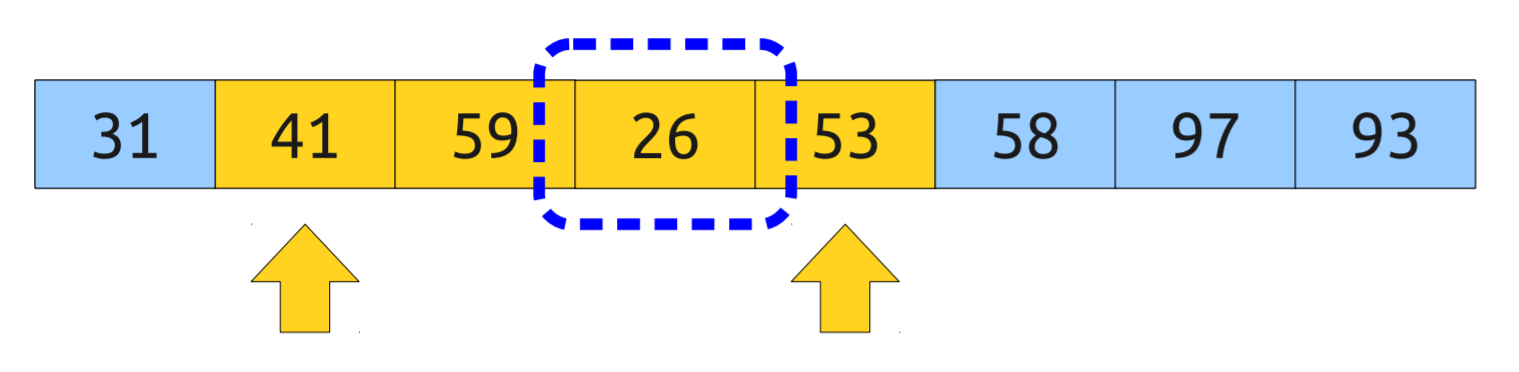
\includegraphics[height=3cm]{Term_2/Source/images/9-rmq.png}
\end{center}

\end{frame}

\begin{frame}[fragile]{Задача RMQ}

\textbf{Разновидности задач}\\
По количеству запросов:
\begin{itemize}
    \item offline - можно получить много запросов, проанализировать их все и выдать ответ на все сразу
    \item online - обработка запросов строго по одному
\end{itemize}
По возможности измнения исходного массива:
\begin{itemize}
    \item static - массив чисел закреплён
    \item dynamic - массив чисел меняется
\end{itemize}
\end{frame}

\begin{frame}[fragile]{Online vs offline}
\begin{center}
    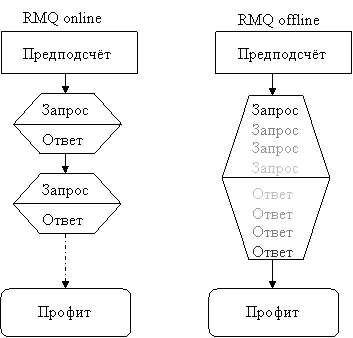
\includegraphics[height=6.5cm]{Term_2/Source/images/rmq1.png}
\end{center}
\end{frame}

\begin{frame}[fragile]{Тривиальное решение}

\begin{enumerate}
    \item Без предобработки \\
Время препроцессинга: O(1)\\
Время ответа: O(n)\\
    \item С предобработкой\\
Время препроцессинга: O($n^3$)\\
Время ответа: O(1)\\
Нужно вычислить $n^2$ возможных отвезков, каждый вычисляем за n.
\begin{center}
    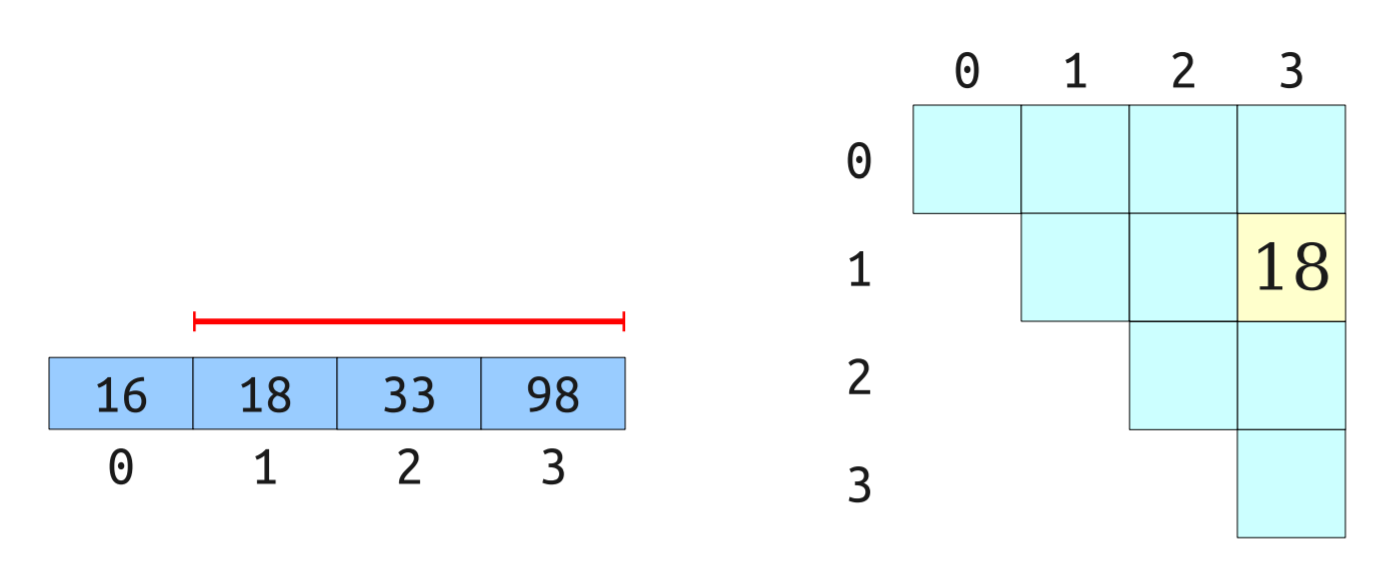
\includegraphics[height=3cm]{Term_2/Source/images/9-rmq-2.png}
\end{center}
\textbf{Замечание}: $n^3$ может быть сокращен до $n^2$ с помощью динамики
\end{enumerate}

\end{frame}


\section{Sqrt-декомопзиция}

\begin{frame}[fragile]{Sqrt-декомопзиция}
Поделим массив на блоки размером $\sqrt{n}$. Предпосчитаем минимумы на этих блоках.
\begin{center}
    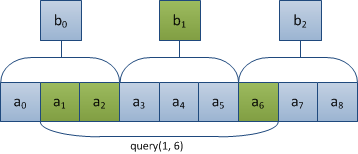
\includegraphics[height=3cm]{Term_2/Source/images/rmq-sqrt.png}
\end{center}
При запросе берём минимум из минимумов полностью покрытых блоков и оставшихся элементов неполностью покрытых блоков.
\end{frame}

\begin{frame}[fragile]{Sqrt-декомопзиция}
Время препроцессинга: O(n)\\
Время ответа: O($\sqrt{n}$)\\
\end{frame}

\section{Sparse table}

\begin{frame}[fragile]{Sparse table - цель}
Проблема: время на ответ у sqrt-декомпозиции все еще очень долгое. \\
Хотим: немного увеличим время на препроцессинг, но добьёмся константного времени на ответ. \\
Цель: \\
Препроцессинг - O( n log n ), \\
Запрос - O(1)
\end{frame}

\begin{frame}[fragile]{Sparse table - интуиция}
Нам не обязательно вычислять все $n^2$ интервалов, чтобы уметь отвечать про минимум за O(1). Каждый интервал может быть накрыт двумя интервалами длины степени двойки.\\
\begin{center}
    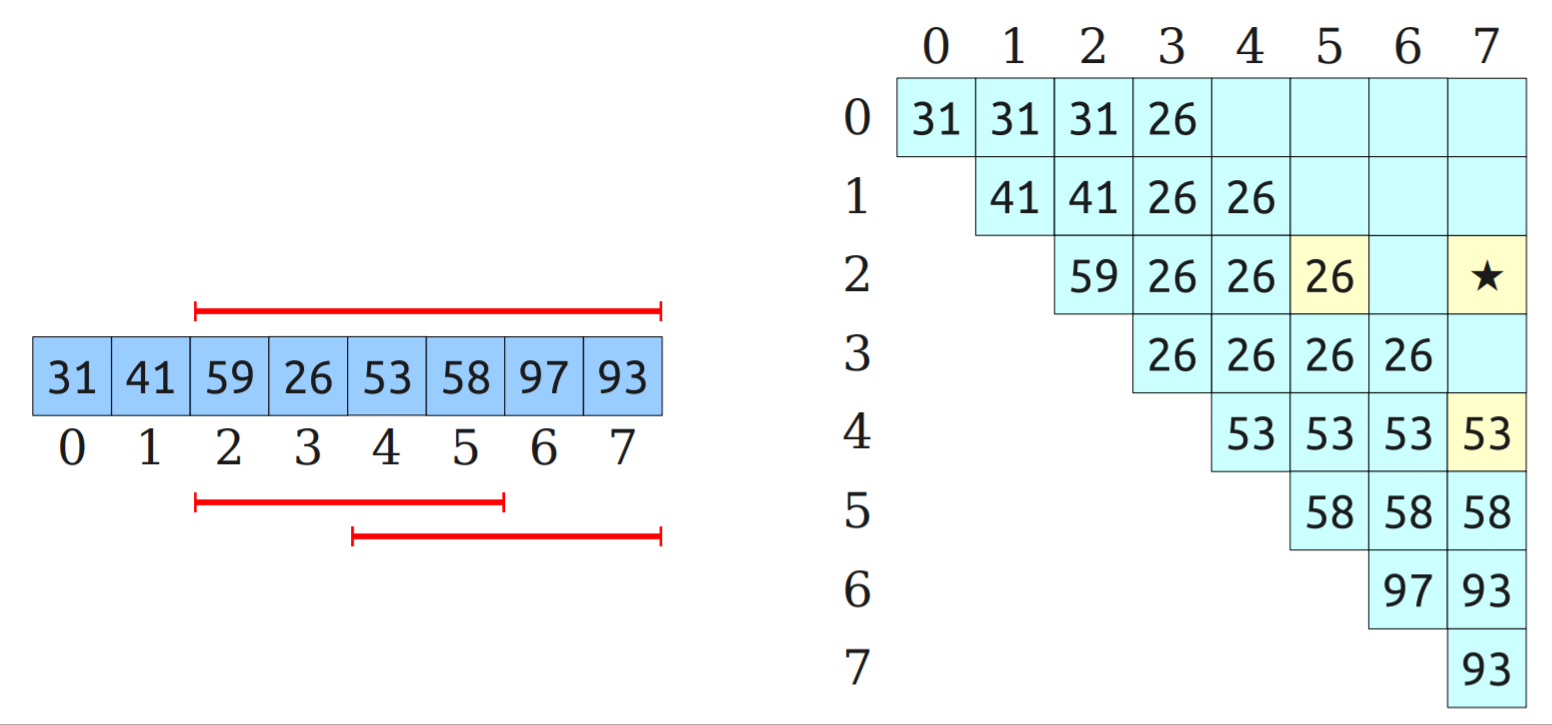
\includegraphics[height=4cm]{Term_2/Source/images/9-sparse-3.png}
\end{center}
\end{frame}

\begin{frame}[fragile]{Sparse table - описание идеи}
Заведем таблицу ST, такую, что она содержит минимумы на всех отрезках, длина которых есть степень двойки.\\
Имеем $n*log(n)$ интервалов, которые можно вычислить за $n*log(n)$ с помощью динамического программирования
\begin{center}
    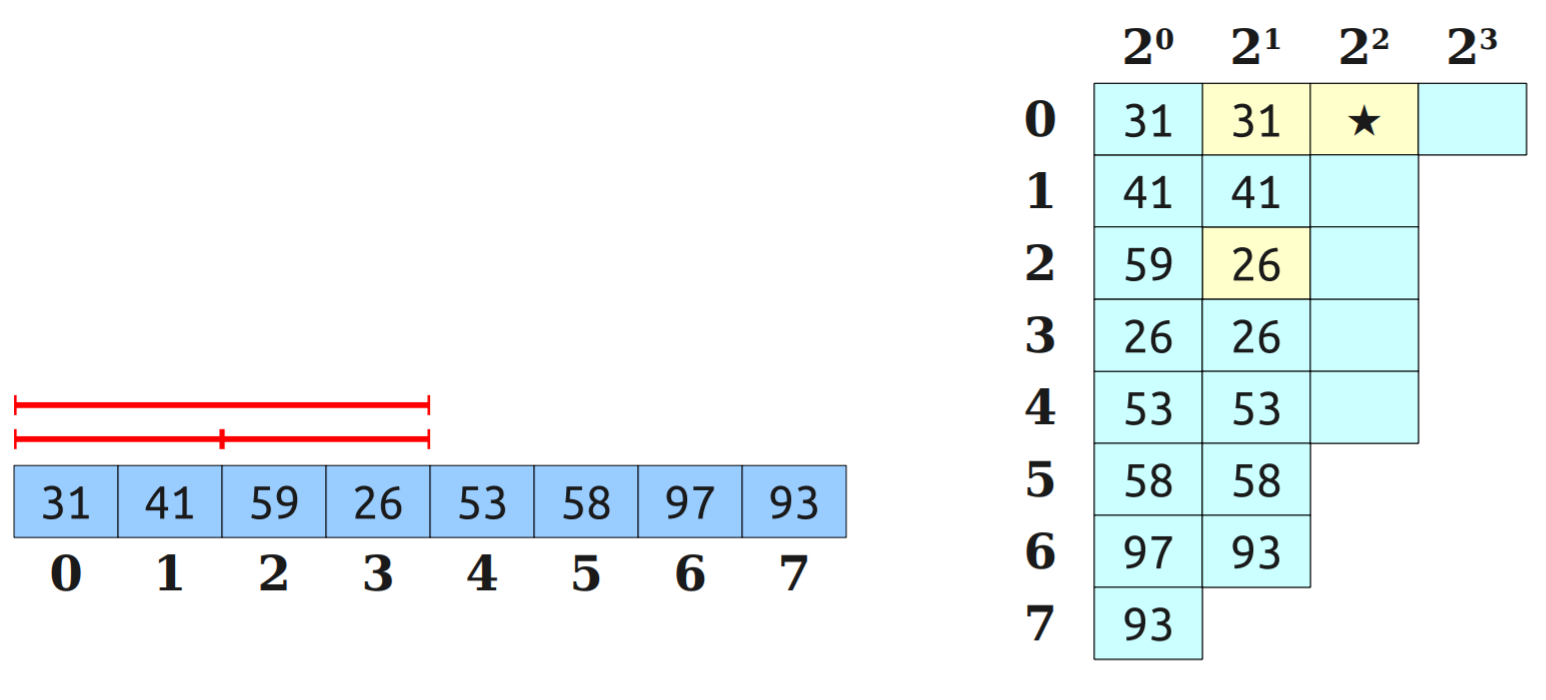
\includegraphics[height=4cm]{Term_2/Source/images/9-sparse-4.png}
\end{center}
\end{frame}

\begin{frame}[fragile]{Sparse table - реализация препроцессинга}
Дано: массив A \\
Таблица $ST[k][i] = min$ на полуинтервале $[ A[i], A[i+2^k] )$. \\
Формула для вычисления таблицы с помощью динамики:\\
$ST[k][i] = min( ST[k-1][i], ST[k-1][i + 2^(k-1)] )$. \\
Благодаря ей мы можем сначала посчитать ST[0], ST[1], потом ST[2] и т.д.
\begin{center}
    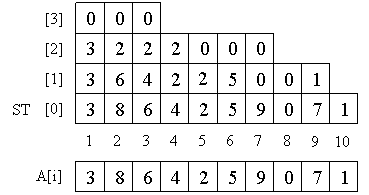
\includegraphics[height=4cm]{Term_2/Source/images/9-sparse-2.png}
\end{center}
\end{frame}

\begin{frame}[fragile]{Sparse table - как вычислять запрос?}
$RMQ(i,j) = min (ST[k][i], ST[k][ j - 2^k + 1]$ \\
$k = log( j-i+1)$ \\
Например, \\
$RMQ(1,6) = min ( ST[2][1] + ST[2][6-4+1])$
\begin{center}
    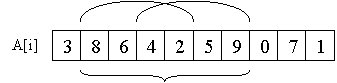
\includegraphics[height=2cm]{Term_2/Source/images/9-sparse-1.png}
\end{center}
\end{frame}

\begin{frame}[fragile]{Sparse table - оценка работы}
Оценки работы: \\
Препроцессинг - O( n log n ), \\
Запрос - O(1)
\end{frame}

\section{Дерево отрезков}

\begin{frame}[fragile]{Дерево отрезков}
Рассмотрим еще одну структуру данных для решения задачи RMQ\\
Дерево отрезков -- это двоичное дерево, в каждой вершине которого написано значение заданной функции на некотором отрезке. Функция в нашем случае – это минимум. 
\begin{center}
    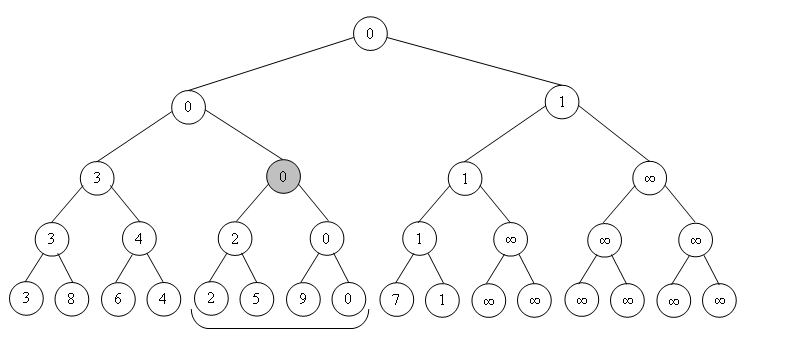
\includegraphics[height=4cm]{Term_2/Source/images/9-segment-tree-0.png}
\end{center}
\end{frame}

\begin{frame}[fragile]{Дерево отрезков - построение и хранение}
Как храним дерево?\\
Храним подобно бинарной куче - заведём массив $T[2n – 1]$. \\
Свойства:
\begin{itemize}
    \item Корень будет лежать в первом элементе массива
    \item Листы лежат в элементах с номерами от $n$ до $2n-1$. 
    \item Сыновья $i$-ой вершины будут лежать в элементах с номерами $2i$ и $2i + 1$ – левый и правый соответственно.
    \item $T[i] = min(T[2i], T[2i + 1])$ для i-ой вершины, не являющейся листом. 
\end{itemize}
Построение за O(n) подобно бинарной куче.
\end{frame}

\begin{frame}[fragile]{Дерево отрезков - вычисление}
Фундаментальный отрезок -- такой отрезок, что существует вершина в дереве, которой он соответствует. \\
\textbf{Утверждение}: на каждом уровне их количество не превосходит 2. 
\begin{center}
    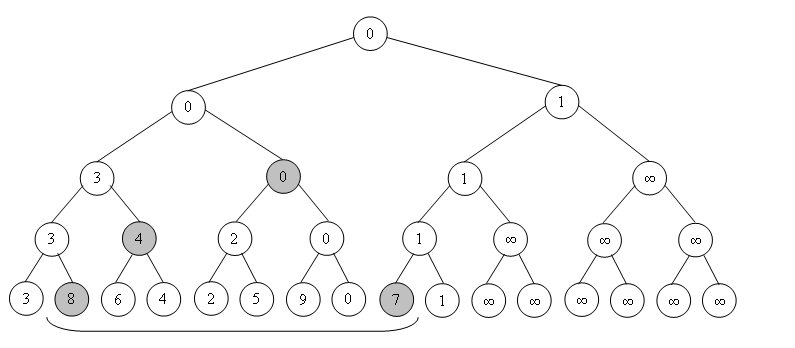
\includegraphics[height=4cm]{Term_2/Source/images/9-segment-tree-1.png}
\end{center}
\end{frame}

\begin{frame}[fragile]{Дерево отрезков - вычисление}
Два способа вычисления решения:
\begin{itemize}
    \item Вычисление сверху
    \item Вычисление снизу
\end{itemize}
\begin{center}
    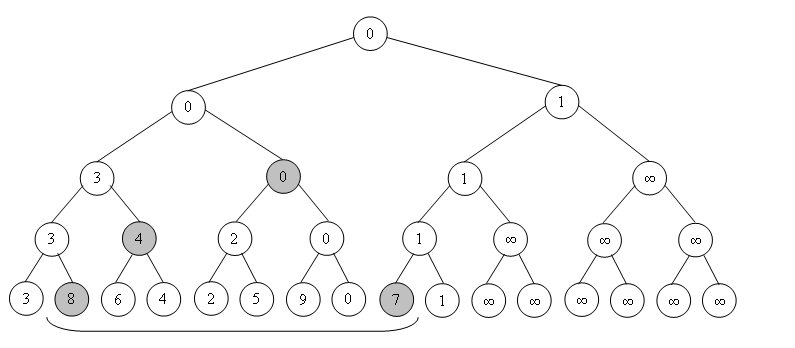
\includegraphics[height=4cm]{Term_2/Source/images/9-segment-tree-1.png}
\end{center}
\end{frame}

\begin{frame}[fragile]{Дерево отрезков - вычисление сверху}
Алгоритм. Начнем проверять детей вершины root. \\
Возможны два варианта: 
\begin{itemize}
    \item отрезок [l \ldots r] попадает только в одного сына корня.\\
    Просто перейдём в того сына, в котором лежит наш отрезок-запрос, и применим описываемый здесь алгоритм к текущей вершине.
    \item отрезок пересекается с обоими сыновьями. Перейти сначала в левого сына и посчитать ответ на запрос в нём, а затем — перейти в правого сына, посчитать в нём ответ и выбрать min(max).
\end{itemize}
\begin{center}
    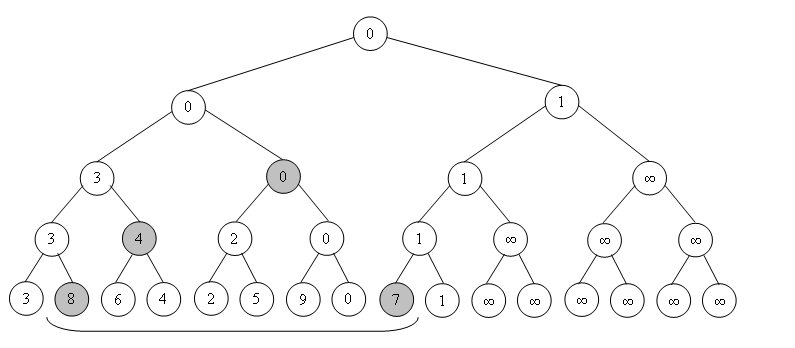
\includegraphics[height=4cm]{Term_2/Source/images/9-segment-tree-1.png}
\end{center}
\end{frame}

\begin{frame}[fragile]{Дерево отрезков - вычисление снизу}
Заведём два указателя – l и r. Изначально установим l и r указывающими на листы, соответствующие концам отрезка запроса. \\
Заметим, что если l указывает на вершину, являющуюся правым сыном своего родителя, то эта вершина принадлежит разбиению на фундаментальные отрезки, в противном случае не принадлежит. Аналогично с указателем r – если он указывает на вершину, являющуюся левым сыном своего родителя, то добавляем её в разбиение. После этого сдвигаем оба указателя на уровень выше и повторяем операцию. Продолжаем операции пока указатели не зайдут один за другой.
\begin{center}
    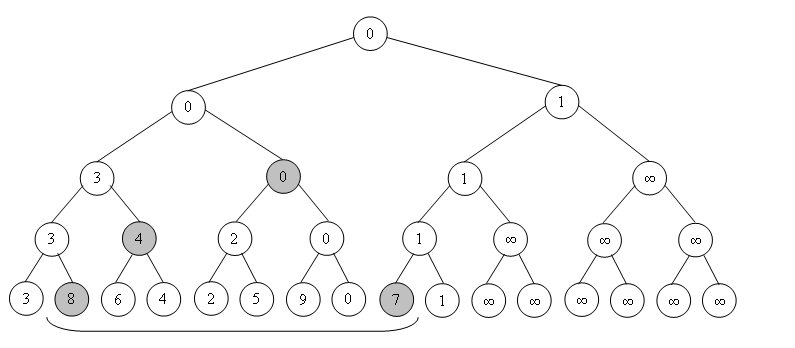
\includegraphics[height=3cm]{Term_2/Source/images/9-segment-tree-1.png}
\end{center}
\end{frame}

\begin{frame}[fragile]{Дерево отрезков - вычисление снизу}
\begin{center}
    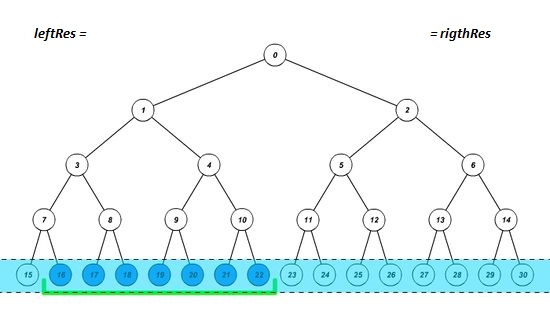
\includegraphics[height=6cm]{Term_2/Source/images/9-up-1.jpg}
\end{center}
\end{frame}

\begin{frame}[fragile]{Дерево отрезков - вычисление снизу}
\begin{center}
    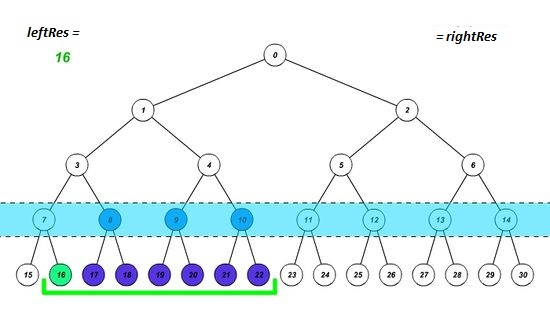
\includegraphics[height=6cm]{Term_2/Source/images/9-up-2.jpg}
\end{center}
\end{frame}

\begin{frame}[fragile]{Дерево отрезков - вычисление снизу}
\begin{center}
    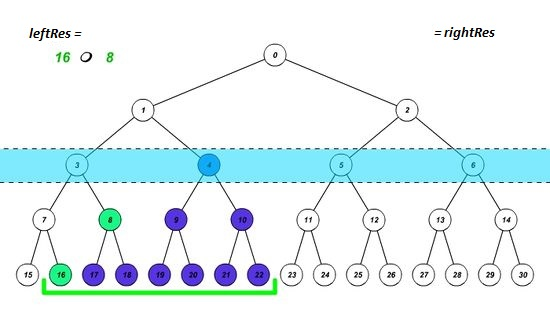
\includegraphics[height=6cm]{Term_2/Source/images/9-up-3.jpg}
\end{center}
\end{frame}

\begin{frame}[fragile]{Дерево отрезков - вычисление снизу}
\begin{center}
    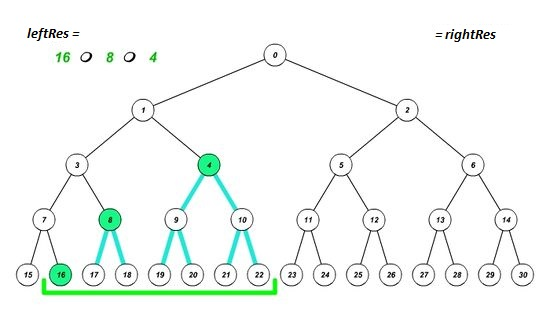
\includegraphics[height=6cm]{Term_2/Source/images/9-up-4.jpg}
\end{center}
\end{frame}

\begin{frame}[fragile]{Дерево отрезков - модификация}
Как изменить значение элемента дерева? Заметим, что для каждого листа есть ровно $log(n)$ фундаментальных отрезков, которые его содержат – все они соответствуют вершинам, лежащим на пути от нашего листа до корня.\\
Значит, при изменении элемента достаточно просто пробежаться от его листа до корня и обновить значение во всех вершинах на пути по формуле $T[i] = min(T[2i], T[2i + 1])$. 
\begin{center}
    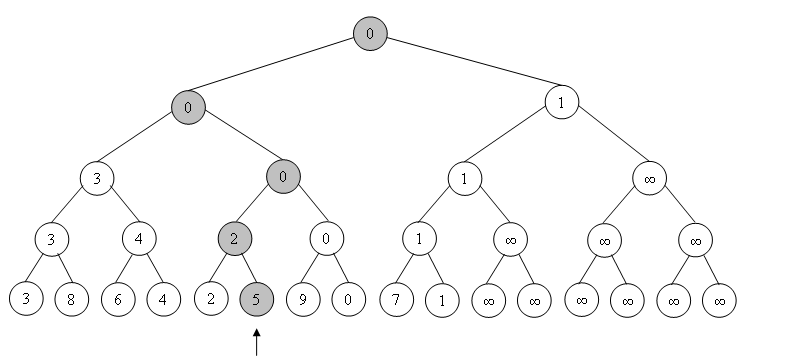
\includegraphics[height=4cm]{Term_2/Source/images/9-segment-tree-2-modif.png}
\end{center}
\end{frame}

\begin{frame}[fragile]{Дерево отрезков - оценка работы}
Оценки работы: \\
Препроцессинг - O(n) \\
Запрос - O(logn)).
\end{frame}

\begin{frame}[fragile]{Дерево отрезков - максимальная сумма на подотрезке}

Введём для каждой вершины 4 числа:\\
\begin{itemize}
    \item Сумма на отрезке
    \item Максимальная из сумм на префисках отрезка:
    \item Максимальная из сумм на суффиксах отрезка
    \item Максимальная сумма на подотрезке
\end{itemize}
Шаг (из $[l_1, r_1], [l_2, r_2]$ собираем $[l_1, r_2]$):
\begin{itemize}
    \item $S(l_1, r_2) = sum(S(l_1, r_1), S(l_2, r_2))$
    \item $Pr(l_1, r_2) = max(Pr(l_1, r_1), S(l_1, r_1) + Pr(l_2, r_2))$
    \item $Suf(l_1, r_2) = max(Suf(l_2, r_2), S(l_2, r_2) + Suf(l_1, r_1))$
    \item $R(l_1, r_2) = max(R(l_2, r_2), R(l_1, r_1), Pr(l_2, r_2) + Suf(l_1, r_1))$
\end{itemize}
\end{frame}


\appendix

\begin{frame}[allowframebreaks]
  \frametitle<presentation>{Полезные ссылки}
    
  \begin{thebibliography}{10}
{
  \beamertemplatebookbibitems
  % Start with overview books.

  \bibitem{emaxx}
  \texttt{E-maxx: sqrt-декомпозиция}
  \newblock \href{https://e-maxx.ru/algo/sqrt_decomposition}
  {\texttt{https://e-maxx.ru/algo/sqrt_decomposition}}
 
  \bibitem{Static RMQ}
  \texttt{Хабр: Static RMQ}
  \newblock \href{https://habr.com/ru/post/114980/}
  {\texttt{https://habr.com/ru/post/114980/}}
  
}
  \end{thebibliography}
  \end{frame}

\end{document}


